Αυτή η ενότητα παρουσιάζει τα αποτελέσματα απόδοσης του αλγορίθμου MinBFT-SGX με τη χρήση micro-benchmarks. Μετρήσαμε την καθυστέρηση και την απόδοση των εφαρμογών MinBFT με μηδενικές λειτουργίες. Το PBFT θεωρείται συχνά ως η γραμμή βάσης για τους αλγόριθμους BFT, επομένως μας ενδιαφέρει η σύγκριση της δικής μας υλοποίησης του αλγορίθμου με την εφαρμογή που είναι διαθέσιμη στο web. Για να συγκρίνουμε αυτή την εφαρμογή με τον αλγόριθμο MinBFT-SGX, χρησιμοποίησα την υλοποίηση της κανονικής λειτουργίας του PBFT στην Java (JPBFT).
Αυτή η ενότητα παρουσιάζει τα αποτελέσματα απόδοσης του αλγορίθμου MinBFT-SGX με τη χρήση micro-benchmarks. Μετρήσαμε την καθυστέρηση και την απόδοση των εφαρμογών MinBFT με μηδενικές λειτουργίες. Το PBFT θεωρείται συχνά ως η γραμμή βάσης για τους αλγόριθμους BFT, επομένως μας ενδιαφέρει η σύγκριση της δικής μας υλοποίησης του αλγορίθμου με την εφαρμογή που είναι διαθέσιμη στο web. Για να συγκρίνουμε αυτή την εφαρμογή με τον αλγόριθμο MinBFT-SGX, χρησιμοποίησα την υλοποίηση της κανονικής λειτουργίας του PBFT στην Java (JPBFT).
Αυτή η ενότητα παρουσιάζει τα αποτελέσματα απόδοσης του αλγορίθμου MinBFT-SGX με τη χρήση micro-benchmarks. Μετρήσαμε την καθυστέρηση και την απόδοση των εφαρμογών MinBFT με μηδενικές λειτουργίες. Το PBFT θεωρείται συχνά ως η γραμμή βάσης για τους αλγόριθμους BFT, επομένως μας ενδιαφέρει η σύγκριση της δικής μας υλοποίησης του αλγορίθμου με την εφαρμογή που είναι διαθέσιμη στο web. Για να συγκρίνουμε αυτή την εφαρμογή με τον αλγόριθμο MinBFT-SGX, χρησιμοποίησα την υλοποίηση της κανονικής λειτουργίας του PBFT στην Java (JPBFT).

\section{Micro-Benchmarks}
Αυτή η ενότητα παρουσιάζει τα αποτελέσματα απόδοσης του αλγορίθμου MinBFT-SGX με τη χρήση micro-benchmarks. Μετρήσαμε την καθυστέρηση και την απόδοση των εφαρμογών MinBFT με μηδενικές λειτουργίες. Το PBFT θεωρείται συχνά ως η γραμμή βάσης για τους αλγόριθμους BFT, επομένως μας ενδιαφέρει η σύγκριση της δικής μας υλοποίησης του αλγορίθμου με την εφαρμογή που είναι διαθέσιμη στο web. Για να συγκρίνουμε αυτή την εφαρμογή με τον αλγόριθμο MinBFT-SGX, χρησιμοποίησα την υλοποίηση της κανονικής λειτουργίας του PBFT στην Java (JPBFT).

Αυτή η ενότητα παρουσιάζει τα αποτελέσματα απόδοσης του αλγορίθμου MinBFT-SGX με τη χρήση micro-benchmarks. Μετρήσαμε την καθυστέρηση και την απόδοση των εφαρμογών MinBFT με μηδενικές λειτουργίες. Το PBFT θεωρείται συχνά ως η γραμμή βάσης για τους αλγόριθμους BFT, επομένως μας ενδιαφέρει η σύγκριση της δικής μας υλοποίησης του αλγορίθμου με την εφαρμογή που είναι διαθέσιμη στο web. Για να συγκρίνουμε αυτή την εφαρμογή με τον αλγόριθμο MinBFT-SGX, χρησιμοποίησα την υλοποίηση της κανονικής λειτουργίας του PBFT στην Java (JPBFT).

\section{End-to-End Benchmarks (Latency)}
Αυτή η ενότητα παρουσιάζει τα αποτελέσματα απόδοσης του αλγορίθμου MinBFT-SGX με τη χρήση micro-benchmarks. Μετρήσαμε την καθυστέρηση και την απόδοση των εφαρμογών MinBFT με μηδενικές λειτουργίες. Το PBFT θεωρείται συχνά ως η γραμμή βάσης για τους αλγόριθμους BFT, επομένως μας ενδιαφέρει η σύγκριση της δικής μας υλοποίησης του αλγορίθμου με την εφαρμογή που είναι διαθέσιμη στο web. Για να συγκρίνουμε αυτή την εφαρμογή με τον αλγόριθμο MinBFT-SGX, χρησιμοποίησα την υλοποίηση της κανονικής λειτουργίας του PBFT στην Java (JPBFT).

\vspace{0.3cm}

\begin{table}[h!]
\centering
\begin{tabular}{ | c | c | c | c |}
 \hline
 \multicolumn{4}{|c|}{Μετρήσεις Latency} \\
 \hline
 Req/Res & JPBFT & MinBFT-SGX Hardware Mode & MinBFT-SGX Simulation Mode\\
 \hline
 0/0 & 0.55 ms & 1339.46 ms & 1.3 ms\\
 4K/0 & 0.55 ms & 1432.68 ms & 1.40 ms\\
 0/4k & 0.57 ms & 1546.67 ms & 1.45 ms\\
 \hline
\end{tabular}
\caption{Καθυστέρηση για διάφορα μεγέθη Αίτησης και Απάντησης για το JPBFT και το MinBFT-SGX}
\label{table:latency}
\end{table}

%\vspace{0.4cm}

Αυτή η ενότητα παρουσιάζει τα αποτελέσματα απόδοσης του αλγορίθμου MinBFT-SGX με τη χρήση micro-benchmarks. Μετρήσαμε την καθυστέρηση και την απόδοση των εφαρμογών MinBFT με μηδενικές λειτουργίες. Το PBFT θεωρείται συχνά ως η γραμμή βάσης για τους αλγόριθμους BFT, επομένως μας ενδιαφέρει η σύγκριση της δικής μας υλοποίησης του αλγορίθμου με την εφαρμογή που είναι διαθέσιμη στο web. Για να συγκρίνουμε αυτή την εφαρμογή με τον αλγόριθμο MinBFT-SGX, χρησιμοποίησα την υλοποίηση της κανονικής λειτουργίας του PBFT στην Java (JPBFT).


\section{Αξιολόγηση του MinBFT-SGX (Throughput)}
Αυτή η ενότητα παρουσιάζει τα αποτελέσματα απόδοσης του αλγορίθμου MinBFT-SGX με τη χρήση micro-benchmarks. Μετρήσαμε την καθυστέρηση και την απόδοση των εφαρμογών MinBFT με μηδενικές λειτουργίες. Το PBFT θεωρείται συχνά ως η γραμμή βάσης για τους αλγόριθμους BFT, επομένως μας ενδιαφέρει η σύγκριση της δικής μας υλοποίησης του αλγορίθμου με την εφαρμογή που είναι διαθέσιμη στο web. Για να συγκρίνουμε αυτή την εφαρμογή με τον αλγόριθμο MinBFT-SGX, χρησιμοποίησα την υλοποίηση της κανονικής λειτουργίας του PBFT στην Java (JPBFT).
Το Σχήμα \ref{fig:JPBFTvsMinBFT} δείχνει ότι τα λιγότερα βήματα επικοινωνίας και ο αριθμός των αντιγράφων στο MinBFT-SGX αντικατοπτρίζεται σε υψηλότερη απόδοση, επιτυγχάνοντας περίπου 30.000 λειτουργίες ανά δευτερόλεπτο. Είναι ενδιαφέρον να παρατηρήσουμε ότι ο μειωμένος αριθμός σταδίων επικοινωνίας και αντιγράφων κάνει τα αντίγραφα(διακομιστές) να επεξεργάζονται λιγότερα μηνύματα (λιγότερα I/O), πράγμα που αυξάνει την απόδοση.

Αυτή η ενότητα παρουσιάζει τα αποτελέσματα απόδοσης του αλγορίθμου MinBFT-SGX με τη χρήση micro-benchmarks. Μετρήσαμε την καθυστέρηση και την απόδοση των εφαρμογών MinBFT με μηδενικές λειτουργίες. Το PBFT θεωρείται συχνά ως η γραμμή βάσης για τους αλγόριθμους BFT, επομένως μας ενδιαφέρει η σύγκριση της δικής μας υλοποίησης του αλγορίθμου με την εφαρμογή που είναι διαθέσιμη στο web. Για να συγκρίνουμε αυτή την εφαρμογή με τον αλγόριθμο MinBFT-SGX, χρησιμοποίησα την υλοποίηση της κανονικής λειτουργίας του PBFT στην Java (JPBFT).

\begin{figure}
\centering
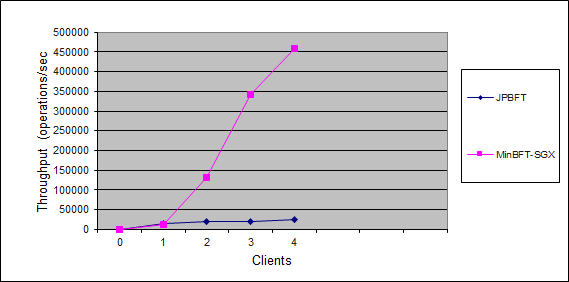
\includegraphics[width=0.8\textwidth]{client_thread_JPBFTvsMinBFT.png}
\caption{Aπόδοση για 0/0 λειτουργίες για το MinBFT και το JPBFT}
\label{fig:JPBFTvsMinBFT}
\end{figure}